\documentclass[11pt]{article}
\usepackage{amsmath,tikz}
\usetikzlibrary{arrows.meta,positioning}
\begin{document}
\section*{T019 / T021 Dependency Map}
\begin{center}
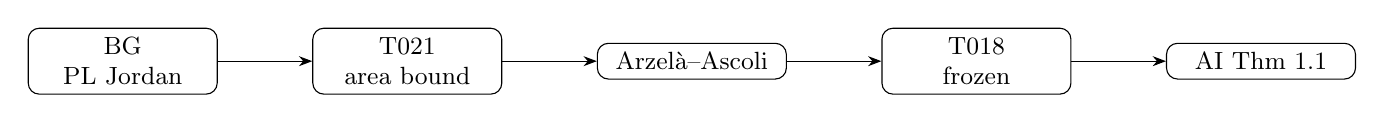
\begin{tikzpicture}[
  node distance=1cm and 1.2cm,
  box/.style={draw,rounded corners,align=center,minimum width=2.4cm,font=\small}
]
  \node[box] (bg) {BG\\PL Jordan};
  \node[box, right=of bg] (t021) {T021\\area bound};
  \node[box, right=of t021] (aa) {Arzel\`a--Ascoli};
  \node[box, right=of aa] (t018) {T018\\frozen};
  \node[box, right=of t018] (ai) {AI Thm 1.1};
  \draw[-{Stealth}] (bg) -- (t021);
  \draw[-{Stealth}] (t021) -- (aa);
  \draw[-{Stealth}] (aa) -- (t018);
  \draw[-{Stealth}] (t018) -- (ai);
\end{tikzpicture}
\end{center}
\end{document}
